\subsection{Measurements with $^{252}$Cf}
\begin{figure}[h]
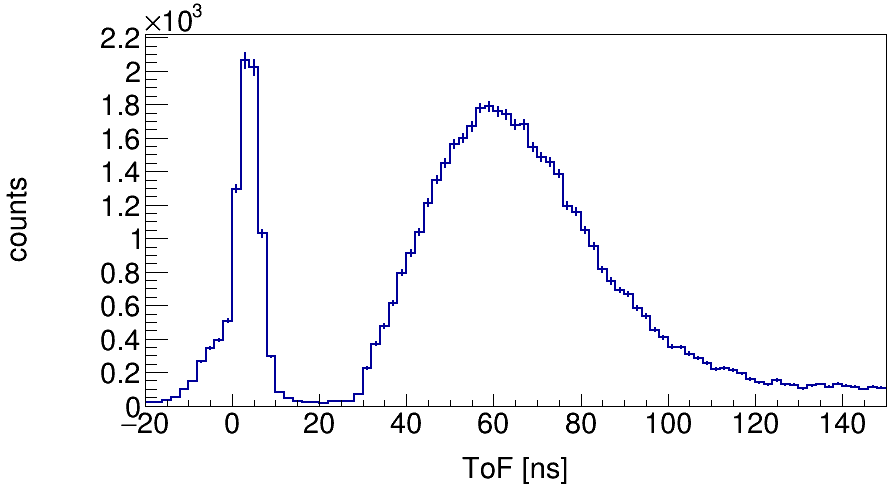
\includegraphics[width=\figsize\textwidth]{Cf252ToF.png}
\caption{Measured ToF spectrum from the SF of $^{252}$Cf. The sharp peak on the left is due to fission photons, followed by another peak due to fission neutrons.}
\label{fig:Cf252ToF}
\end{figure}
A $^{252}$Cf source was placed at the center of the detection system shown in Fig.~\ref{fig:Facility} in order to measure the n-n opening angle distribution.
Several such past measurements have been performed (see Refs.~\cite{1975Cf252, Pozzi2014, 2008CF252, Verbeke2018}), and serve as a means to validate the methods used throughout this study.

The $^{252}$Cf source produces a cleaner ToF spectrum than photofission due to the lack of beam related backgrounds (see Fig.~\ref{fig:Cf252ToF}), and therefore these measurements have a better signal to noise ratio.
Also, there is no concern over the detection of accidental neutron coincidences because the fission rate of the $^{252}$Cf source was about 3,500 fissions/s, making it highly unlikely that multiple fissions will occur during the electronic acceptance time window of 150~ns.
The beginning of the 150~ns neutron acceptance time window was triggered by a 2-fold coincidence, within a 4~ns window, between two separate 10$\times$10$\times$5 cm$^3$ plastic scintillators, one placed above and the other below the source at a distance of 30~cm.
Aside from this difference in the time window triggering mechanism, identical methods were used for both photofission and SF measurements.
\FloatBarrier